\section{Виды моделирования}

\subsection{По признаку характера изучаемых процессов}

\begin{figure}[H]
    \centering
    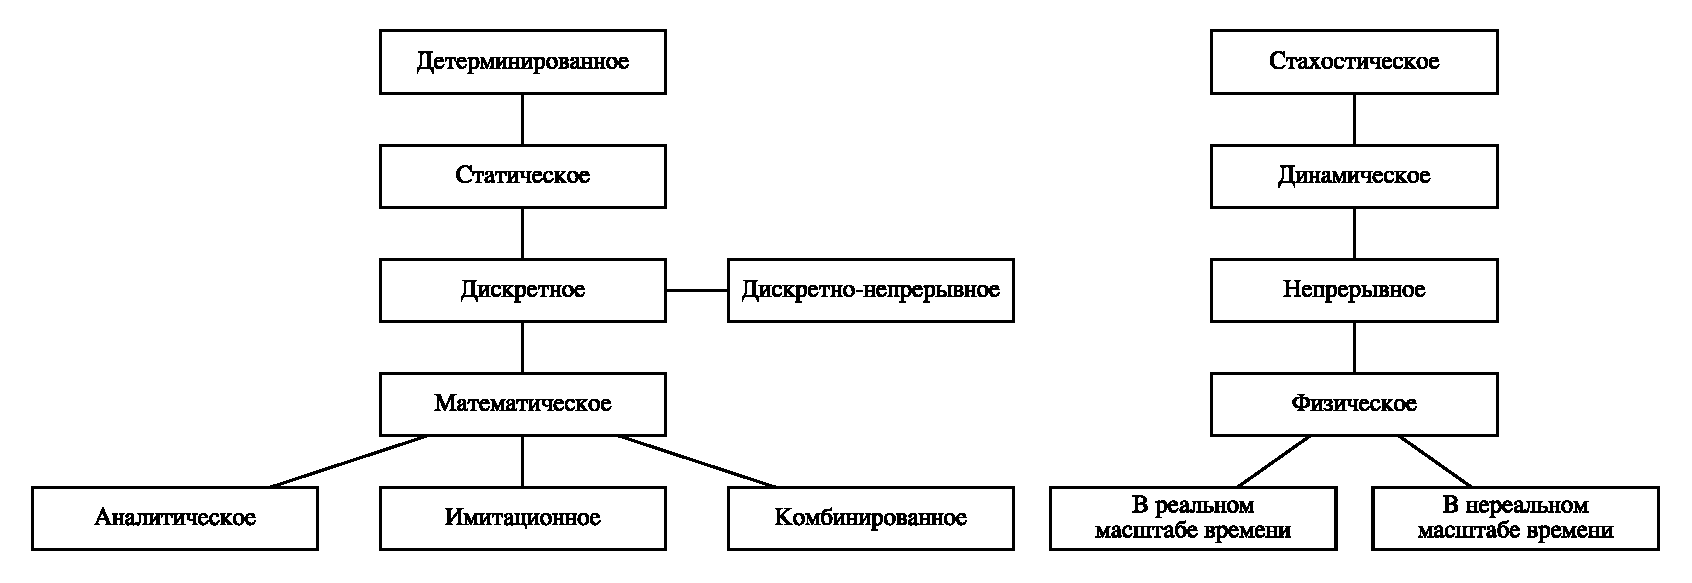
\includegraphics[scale=0.6]{img/content/03_types_modeling/types_modeling.pdf}
    \caption{Виды моделирования}
\end{figure}

Детерминированное моделирование отражает детерминированные процессы, то есть такие, в которых предполагается отсутствие всяких случайных воздействий. Стахостические предполагают наличие случайных воздействий.

Статическое моделирование служит для описания объекта в какой-то момент времени. Динамичсекое отражает поведение объекта во времени.

Дискретное служит для описания процессов, происходящих в дискретные моменты времени, непрерывные -- позволяют отражать непрерывные процессы. Дискретно-непрерывное -- это наличие как дискретных, так и непрерывных компонентов.

Под математическим моделированием будем понимать процесс установления данному реальному объекту некоторого математического объекта, называемого математической моделью и исследований этой модели, позволяющих получить реальные характеристики объекта.

Наглядное моделирование, а именно гипотетическое, аналоговое.

Символическое моделирование: языковое, знаковое.

Математическое: аналитическое, имитационное, комбинированное, информационное, структурное, ситуационное.

Для аналитического моделирования характерно то, что процессы функционирования элементов системы записываются в виде некоторых функциональных соотношений (алгераических, интегро-дифференциальных, конечно-разностных) или логических условий. Аналитическая модель может быть исследована тремя способами

\begin{enumerate}
    \item аналитический -- стремление получить в общем виде зависимости от исходных характеристик;
    \item численный -- нельзя решить уравнение в общем виде получаем решение для каких-то конкретных начальных данных;
    \item качественный -- нет никакой аналитики.
\end{enumerate}

При имитационном моделировании реализующий модель алгоритм воспроизводит процесс функционирования системы во времени, причем имитируются элементарные явления, состовляющие процесс с сохранением их логической структуры и последовательности протекания во времени, что позволяет по исходным данным получить сведения о состоянии процесса в определенные моменты времени, дающие возможность оценить характеристики системы.

Самое главное приемущество аналитического метода -- точность, потому что явно установили зависимость входной характеристики от входной. Имитация используется при невозможности что-либо сделать, создается программная модель.

Основноым приемуществом имитационного моделирования по сравнению с аналитическим является возможность решения более сложных задач. Имитационнные модели позволяют достаточно просто учитывать такие факторы, как наличие дискретных и непрерывных элементов, нелинейные характеристики системы, многочисленные случайные воздействия, что создает значительные трудности при аналитическом моделировании.

Результаты, полученные при имитационном моделировании, являются реализациями случайных величин и функций и, следовательно, нахождение характеристик, происходящих в системе, требует его многократного воспроизведения.

Комбинированное моделирование при анализе систем позволяют объекдинить достоинста отдельных видом моделирования. Обычно проводят декомпозицию процессов поведения объектов на состовляющие подпроцессы и для тех из них, где можно, используюм аналитическую модель.

\subsection{Виды имитационного моделирования}

\begin{itemize}
    \item \textbf{агентное} -- для исследования децентрализованной системы, динамика функционирования которых определяется не глобальными правилами и законами, а наоборот, когда эти глобальные правила и законы являются результатом индивидуальной активности членов группы. Агент -- некая сущность, обладающая активностью, автономным поведением, может принимать решения в соответствиии с некоторым набором правил, взаимодействовать с окружением, а так же самостоятельно изменяться;
    \item \textbf{дискретно-событийное} -- предлагает абстрагироваться от непрерывной природы событий и рассматривать только основные события моделирования системы, например, ожидание, обслуживание заявки и т.д. Сфера приложения: от логистики до систем массового бслуживания (танспортные, производственные).
    \item \textbf{системная динамика} -- парадигма моделирования, где исследуюмей системе ставится в соответсвие графические диаграммы причинных связей и глобальных влияний одних параметров на другие во времени, а затем созданная на основе диаграмм модель программируется. Используется в производстве, развитии города или популяции, в бизнесс-процессах.
\end{itemize}

Имитационнное моделирование является достаточно эффективным, но имеющим свои недостатки. Трудности использования связаны с обеспечением адекватности модели при описании ее как системы, интерперетации результатов, обеспечением стахистической сходимости, решением проблемы размерности, большая трудоемкость методово. Часто перед пстроением имитационной модели, котоая является динамической по своей сути, оказывается полезным, а иногда необходимым осуществить статистический анализ, при этом определяеются и специфируются функции, их взаимосвязи, пототки работ и т.д. Для выполнения такого анализа используют кейс-технологии.

\textbf{Три этапа развития имитационного моделирования} по возможностям для пользователя:

\begin{itemize}
    \item Создание имитационной модели на универсальном ЯП, специализированном или ооп.
    \item Использование при разработке имитационного моделирования проблемно-ориентированных систем. Эти системы не требуют знания программирования, но позволяют моделировать относительно узкий класс задач. Имитационная система генерируется автоматически, тем самым позволяя быстрее созать имитационную модель.
    \item Использование методов искусственного интелекта. Создание интуитивно понятного интеллектуального интерфейса.
\end{itemize}
